\documentclass{article}
\usepackage{enumitem,graphicx,titling,units,braket,amsthm, amsmath,amssymb,mathtools,textcomp,tikz,pgfplots,listings,hyperref, physics, listings, color, float}

\newcommand\numberthis{\addtocounter{equation}{1}\tag{\theequation}}
\allowdisplaybreaks[1]

\makeatletter
\def\myitem{%
   \@ifnextchar[ \@myitem{\@noitemargtrue\@myitem[\@itemlabel]}}
\def\@myitem[#1]{\item[#1]\mbox{}\\\hspace*{\dimexpr-\labelwidth-\labelsep}}
\makeatother

\newtheorem{theorem}{Theorem}
\newtheorem{corollary}[theorem]{Corollary}
\newtheorem{conjecture}[theorem]{Conjecture}

\lstset{
	tabsize=4,
	rulecolor=,
	language=python,
        basicstyle=\scriptsize,
        upquote=true,
        aboveskip={1.5\baselineskip},
        columns=fixed,
        showstringspaces=false,
        extendedchars=true,
        breaklines=true,
        prebreak = \raisebox{0ex}[0ex][0ex]{\ensuremath{\hookleftarrow}},
        frame=single,
        showtabs=false,
        showspaces=false,
        showstringspaces=false,
        identifierstyle=\ttfamily,
        keywordstyle=\color[rgb]{0,0,1},
        commentstyle=\color[rgb]{0.133,0.545,0.133},
        stringstyle=\color[rgb]{0.627,0.126,0.941},
}

\begin{document}
	\setlength{\droptitle}{-10em}
	\title{Homework 5 \& 6}
	\author{Andrew Lei\\Arizona State University}
	\maketitle
	
	\begin{enumerate}
		\item Weights for the first two components of PCA can be found in `data.txt'. Variance explained by component one was about 36.2\%. Variance explained by component two about 19.2\%. Total of first two about 55.4\%.
		\par 
		The true categories for the wine look like this:
		\begin{figure}[H]
		\centering
		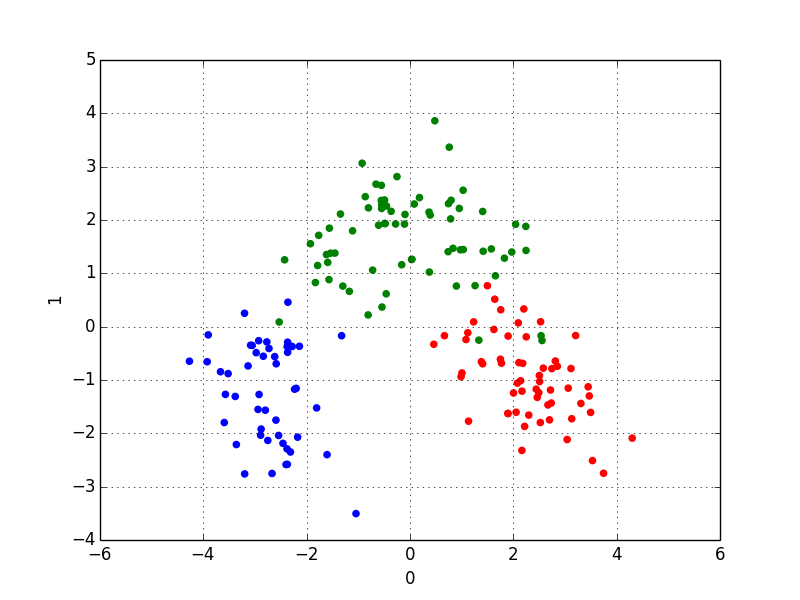
\includegraphics[scale=0.5]{hw5true.png}
		\caption{First two principal components of wine data, colored by type.}
		\end{figure}
		\item Here is the result of running kmeans once:
		\begin{figure}[H]
		\centering
		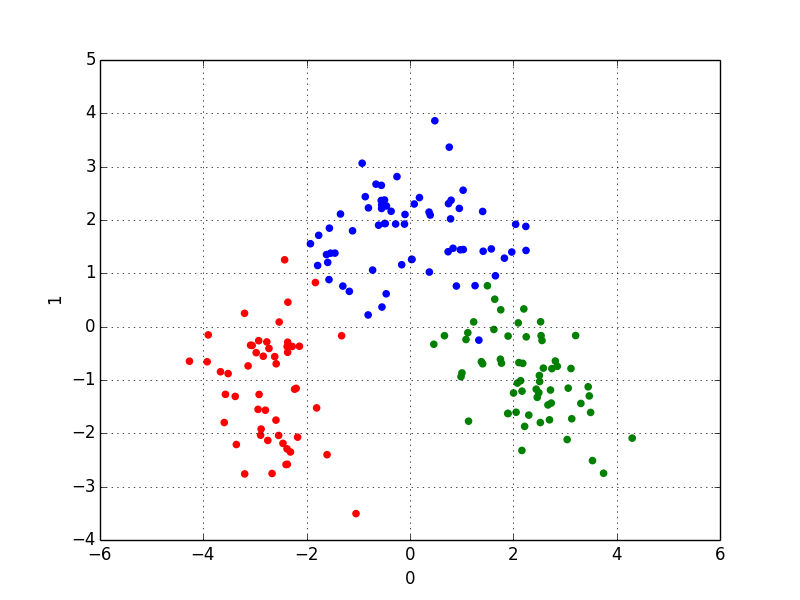
\includegraphics[scale=0.5]{hw5pt2a.png}
		\caption{First two principal components of wine data, clustered using K-means.}
		\end{figure}
		Apart from the different colours, this is quite similar to the above. The points that are different were extracted:
		\begin{figure}[H]
		\centering
		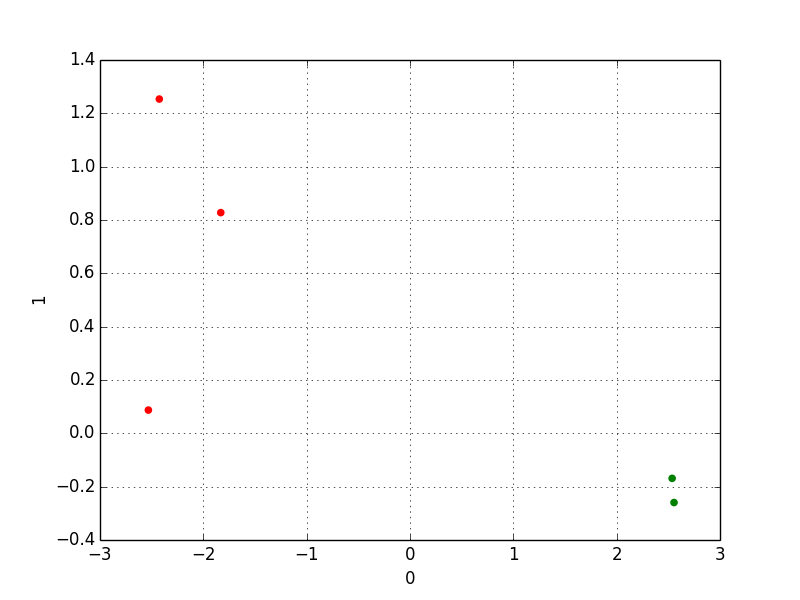
\includegraphics[scale=0.5]{hw5pt2afail.png}
		\caption{First two principal components of wine data, difference between points clustered using K-means and true clusters.}
		\end{figure}
		Images from the ten runs of K-means can be found with the titles of the form `hw5pt2no*.png'. Here is the run with the highest BSS (equivalent to lowest within-cluster-distance):
		\begin{figure}[H]
		\centering
		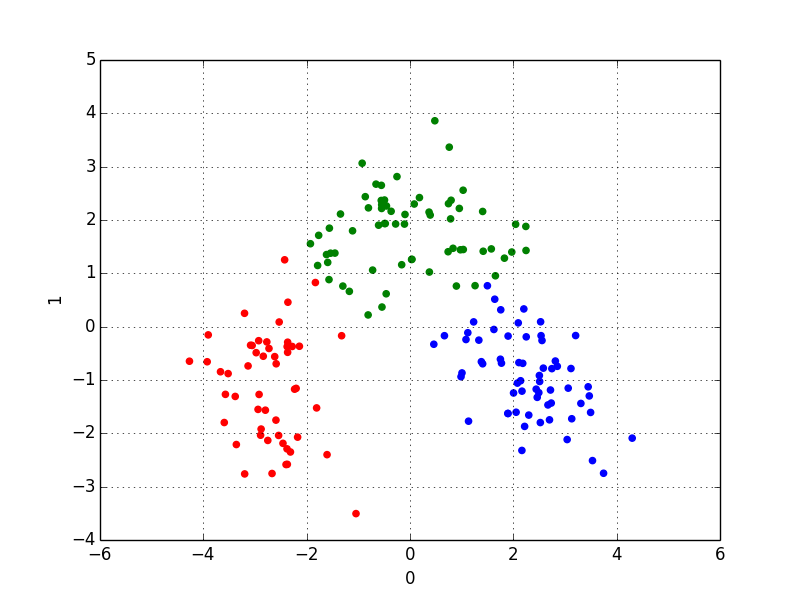
\includegraphics[scale=0.5]{hw5pt2b.png}
		\caption{First two principal components of wine data, clustered using K-means; best of 10.}
		\end{figure}
		And its errors:
		\begin{figure}[H]
		\centering
		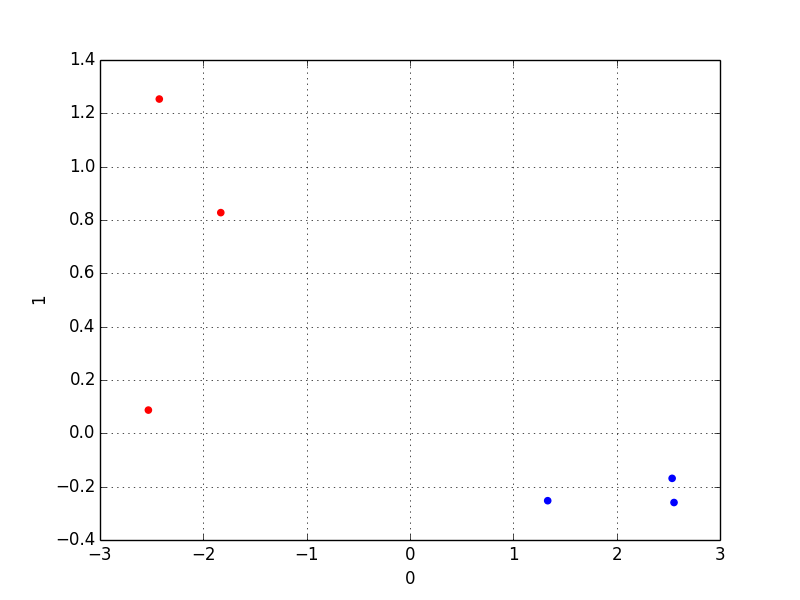
\includegraphics[scale=0.5]{hw5pt2bfail.png}
		\caption{First two principal components of wine data, difference between points clustered using K-means and true clusters; best of 10.}
		\end{figure}
		\item I decided to run these with the same initial starting points as in part 2. Note that in `data.txt' the BSS for these trials are identical to the trials in part 2; it
seems Sci-Kit Learn implements K-means in a manner that results in an identical answer. So while the images are available with the names `hw5pt3no*.png', they don't need much discussion since they are identical to those of the previous section.
		\par
		Note that I have checked the list the keeps track of the initial centroid locations before and after running K-means on it in section 2 to make sure nothing was changed by reference there, so that the initial values used in this section were indeed the same as in section 2.
		\item Single-link was quite bad at clustering the data; most of the data ended up in one large cluster:
		\begin{figure}[H]
			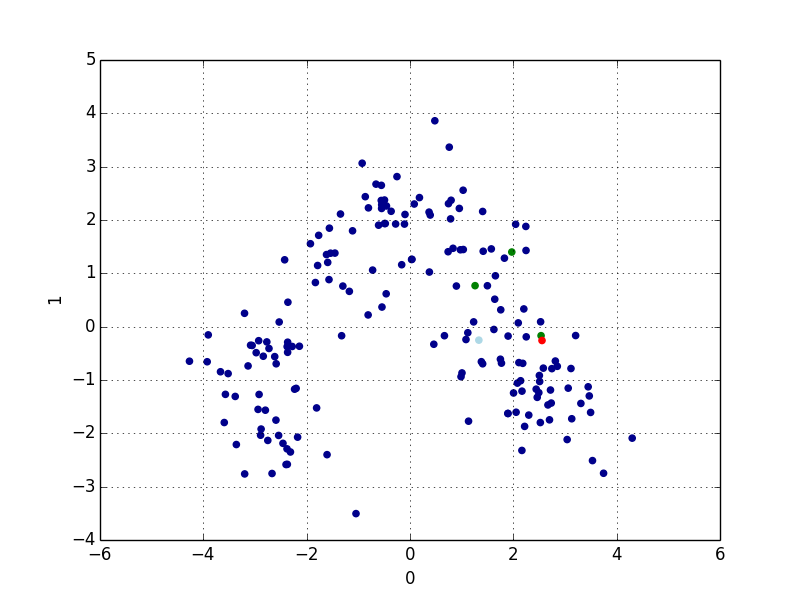
\includegraphics[scale=0.5]{HW6single4.png}
			\caption{Above: Single-link clustering with four clusters. Below: Single-link with three.}
			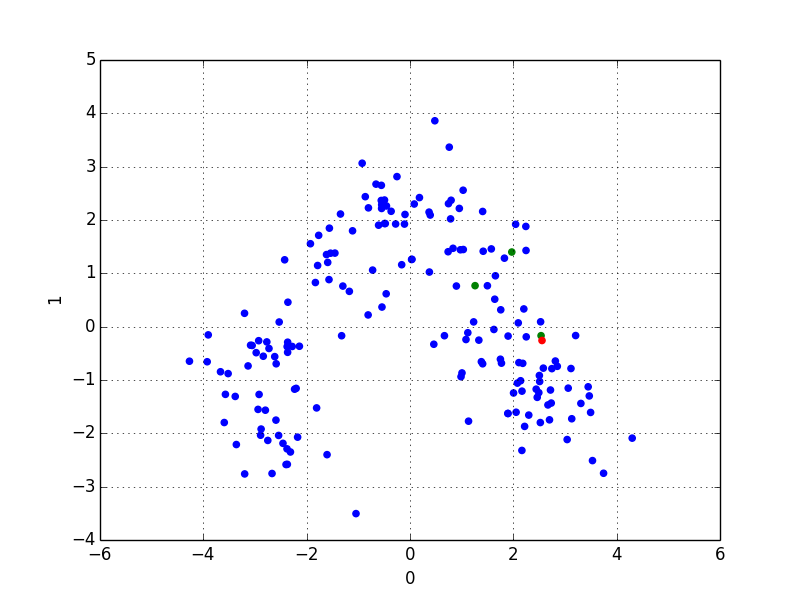
\includegraphics[scale=0.5]{HW6single3.png}
		\end{figure}
		By comparison, complete-link got us closer to the true values:
		\begin{figure}[H]
			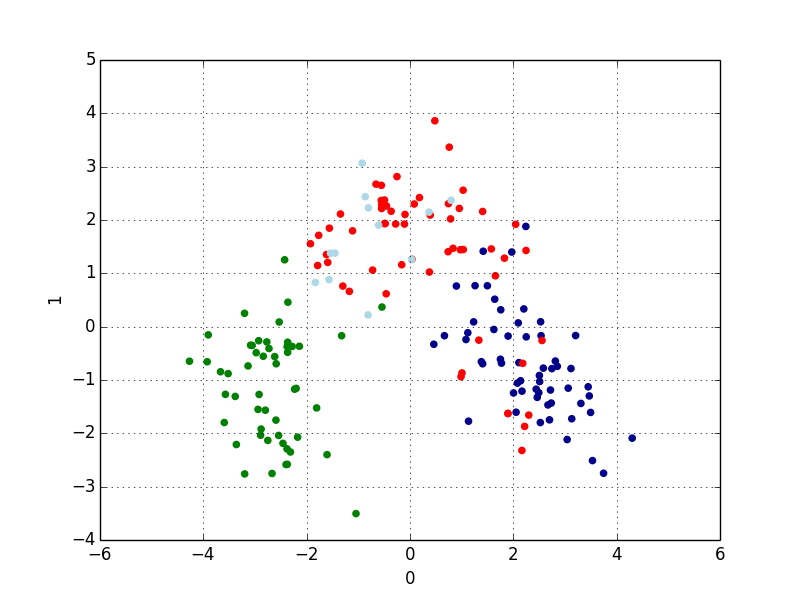
\includegraphics[scale=0.5]{HW6complete4.png}
			\caption{Above: Complete-link clustering with four clusters. Below: Complete-link with three.}
			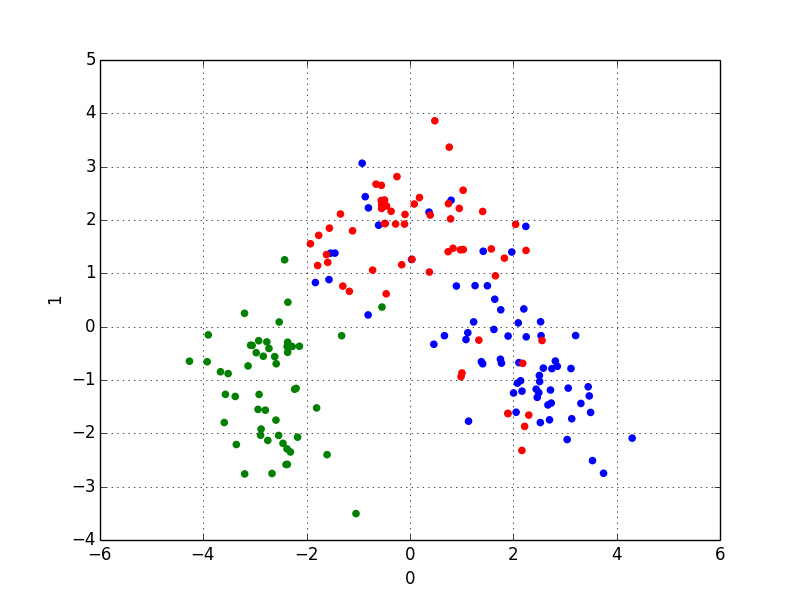
\includegraphics[scale=0.5]{HW6complete3.png}
		\end{figure}
		However, if you note the substantial overlap between the reds and the blues here, it is immediately obvious that this is somewhat poorer than K-means.
		\end{enumerate}
	
\end{document}